\subsection{Attack Vectors}
There are a number of attacks that take advantage of insecurities in the 802.11 standard and that capitalize on unencrypted or WEP encrypted networks. 

\subsubsection{Man in the Middle (MITM)}
The man in the middle attack puts the attacker between the station and the access point, allowing them to eavesdrop on communications taking place. In wireless communications, monitoring passing traffic is trivial considering traffic is broadcast and picked up by all network cards in the vicinity; but usually discarded if not intended recipient. This attack allows the attacker easy access to user data sent over unencrypted protocols such as HTTP, but also allows them to use tools such as sslstrip \cite{research:ssl_strip} to attempt to thwart HTTPS.

\begin{figure}[h!]
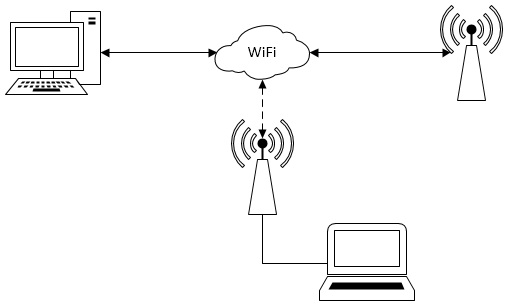
\includegraphics[width=\linewidth]{research/figures/mitm.png}
\caption{Malicious user monitors and injects data packets in to traffic.}
\end{figure}

This style of attack is a popular choice when communications involve some type of public key encryption. 

A more recent variation to this attack, that reflects the shift toward web applications, is the Man in the Browser\footnote{The Boy in the Browser attack \cite{research:bitb} is a less mature version of the Man in the Browser attack. It is a trojan that routes traffic to the attacker’s proxy website to modify before sending to the intended destination.} (MitB). The advantage this has over the vanilla MITM attack is SSL style authentication measures do not hinder its effectiveness. Examples of the MitB attack include HTTP Cache Poisoning \cite{research:cache_poisoning} and HTTP Response Splitting \cite{research:response_splitting}, both can leave lasting effects on the compromised browser.

%This attack will feature in the project implementation as a means of inspecting leaked data from applications when stations are caught in the honeypot.
\subsubsection{Spoof Access Point}
\label{sec:spoofap}
This is not necessarily an attack in itself, but a means of relying on social engineering to gain connections to perform attacks on. A soft access point is a rogue access point that has been established on a wireless adaptor, without the need for a router. Leaving this open, and performing in an area with a high footfall, or cafe area, for example, will allow the attacker to gain connections, monitor traffic, and perform various man-in-the-middle attacks. It can also be paired with other attacks detailed further on in the report.

\begin{figure}[h!]
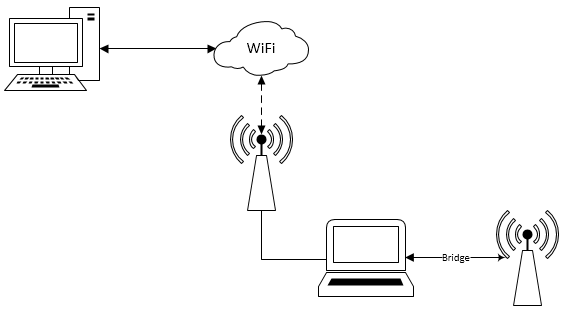
\includegraphics[width=\linewidth]{research/figures/spoofap.png}
\caption{Soft access point bridges traffic to real access point.}
\end{figure}

\subsubsection*{Performing the Attack}
As this is more of a gateway attack, not a lot can be gained from doing it alone. The airbase-ng tool proved the simplest way to create a fake access point, taking the wireless interface and either start or stop as parameters. The image below shows the creation of an access point and a station connecting to it.

\begin{figure}[h!]
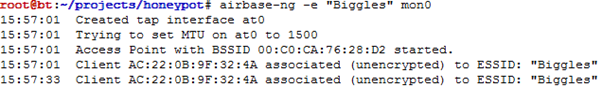
\includegraphics[width=\linewidth]{research/attackvectors/figures/spoofap1.png}
\caption{Soft access point created with the SSID “Biggles”.}
\end{figure}
\subsubsection{HTTP Response Splitting}
\subsubsection{Cafe Latte}
\subsubsection{Deauthentication DOS}
Deauthentication denial of service (DOS) attacks take advantage of either the unencrypted and unauthorized disassociation or deauthentication frames, that originate from either the access point or client, depending on whether the attack wants to block a device or all devices from the network.

When a client wishes to gracefully disconnect from a 802.11 network it sends a deauthentication frame to the access point, likewise when an AP needs to disconnect from a client it sends a disassociation frame. If the AP needs to disconnect all clients, e.g. in the event of a reboot, it broadcasts the disassociation frame. The unencrypted and unauthorized nature of these frames leaves them open to MAC spoofing of either the client or AP, meaning an attacker can easily forge frames. It has been noted that deauthentication frames are preferable to spoof due to the access point and client having to perform the authentication cycle again in order to carry on using the network [1].

\begin{figure}[h!]
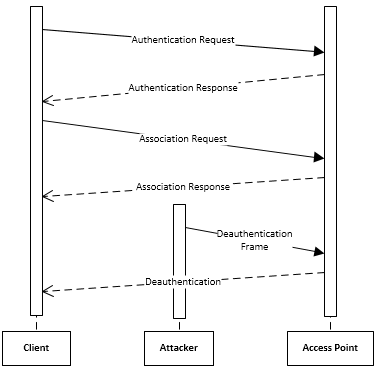
\includegraphics[width=\linewidth]{research/figures/deauthentication.png}
\caption{Deauthentication DOS sequence.}
\end{figure}
\subsubsection{Evil Twin}
The Evil Twin, aka WiFi Phishing, AP Phishing, etc., is another gateway used to leave the target vulnerable to other attacks such as the Man in the Middle detailed previously, stolen security information such as website log in credentials and credit card information, HTTP cache poisoning, DNS poisoning and a whole host more that rely on the victim being on the same network. 

Unsuspecting victims of this attack are forced to connect to a spoofed access point- usually with the same SSID as the real access point- by way of disassociating them with the real AP and having them connect to the fake AP. 

\begin{figure}[h!]
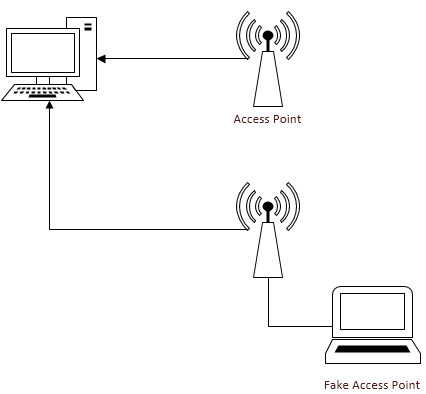
\includegraphics[width=\linewidth]{research/figures/eviltwin.png}
\caption{Fake AP broadcasts at a stronger signal strength.}
\end{figure}

The attacker achieve this by way of two methods. Firstly they need to gain the SSID of access points either through beacon packets, or by probe requests broadcasted by passing devices if the SSID is hidden. Once this is known the attacker can then disconnect users from the real AP through a deauthentication DOS and broadcast the fake AP beacon packets with a stronger signal than the real one. Passing devices sending out probe requests will connect to the AP with the strongest signal, which happens to be the fake one.  

This attack is not thwarted by Wired Equivalent Privacy (WEP) or WiFi Protected Access (WPA) as they only encrypt data after the association is established, thus not protecting against management packet spoofing [1]. There have been efforts made to protect against this attack, not by protecting against MAC spoofing, but by utilising the received signal strength (RSS). This proves a good method of protection for single transmitter source, but it has also been demonstrated to have a 97.8\% success rate with multiple transmitters [3]. 802.11w does implement protected management frames and as a result would eliminate this style of attack.

As noted previously, this attack can leave users open to a faked hotspot login page [2] in which credit card information can be stolen or further chains of attacks.

\subsubsection{Honeypot}
The honeypot attack takes advantage of the Preferred Network List (PNL) that wireless devices maintain once successful connection with an access point has been made. The honeypot attack forms the basis of the program this project is implementing.
